\newpage
\part{Results and Discussion}
This part is organized as follows. First, in the 7th chapter a preliminary analysis is done to characterize the problem and plan the experiments and simulations. Then, in the 8th chapter, the finite element model construction and the simulations are exposed. In the 9th chapter the experiments coupled with the design of experiments methodology are illustrated. Finally, this part is concluded with the discussion in chapter 10 where the main results are put in perspective and compared between simulations and experiments.

\section{Preliminary analysis}

In this first results and discussion chapter I will start by approach by first giving the general context and background of PFS manufacturing in order to understand its components, its function and how they are interlinked. Then, I further investigate the Plunger assembly step and its characterization methods. After, I deconstruct the problem to understand the physics and dividing it into underlying phenomena. Finally, I identify what factors might have an influence on the stages of the assembly and based on the I list the needed experiments and simulations to test the hypothesis and quantify the impact on the process outcome quality (see Figure \ref{fgr:cat}.

\begin{figure}[h!]	
	\centering
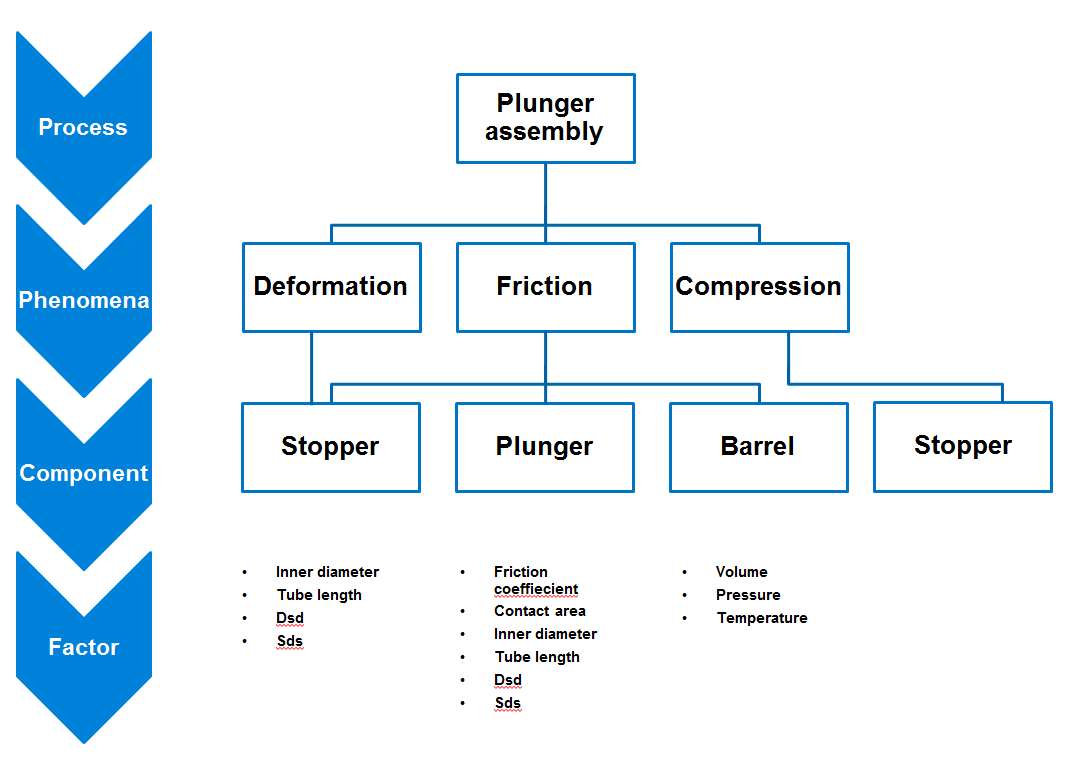
\includegraphics[height=9cm]{img/category.PNG}
   \caption{PR Assembly Step Break-down}
 \label{fgr:cat}
\end{figure}

\newpage
\subsection{Prefilled Syringe manufacturing}

\subsubsection{Components}
The Prefilled Syringe main components are a glass barrel, a rubber stopper, a polymeric tip cap, the liquid medium, a  polymer plunger and a extended finger flange (see Figure \ref{fgr:PFS}). 

\begin{figure}[h]	
	\centering
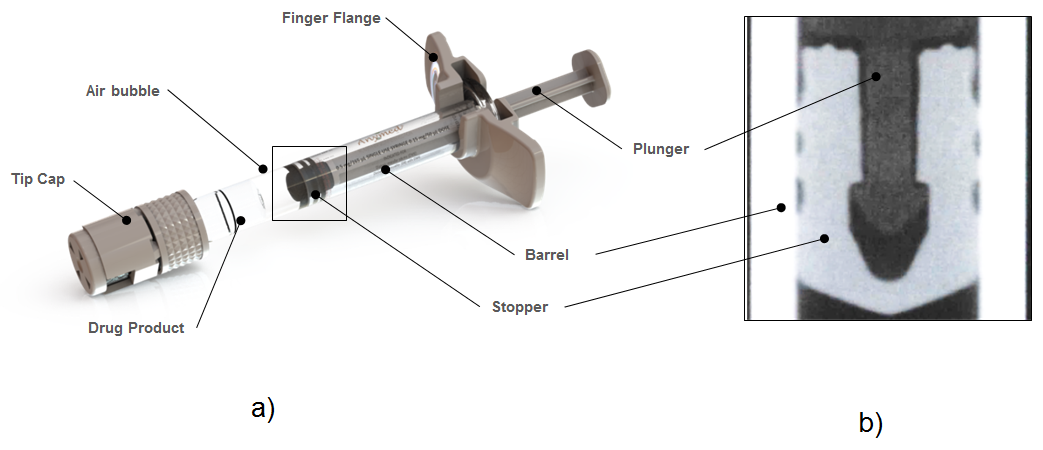
\includegraphics[height=6cm]{img/PFS.PNG}
   \caption{Representation of a) Prefilled  Syringe with described components and b) a Computer Tomography Scan of the Stopper - Plunger snap-fit geometry highlighted in part a).}
 \label{fgr:PFS}
\end{figure}

All of the components can vary depending in design on the requirements but each has a specific role for the drug delivery. A central quality attribute a PFS has to assure is the maintenance of the sterility of the drug product during the whole manufacturing process until it arrives to its end user, the patient. The stopper plays a central role as it provides the barrier separating the medium from the outside. Silicon oil is the invisible component that makes the gears turn as it ensures the isolation, while ensuring the right injection force necessary to deliver the drug. The plunger is the handle, the trigger that enables the administration by pushing downwards the stopper. As described in the problem statement this specific model a snap-fit mechanisms is used to keep the two components together. 

\begin{table}[h]
\def\arraystretch{1.4}
\caption{PFS Components, material composition and fucntion}
	\begin{tabular}{p{2.6cm} p{3.7cm}p{9cm}}
	Components & Material & Function \\
    \hline
Syringe Barrel  & Glass         & Medium container \\
Silicon oil     & Oil           & Lubricant and sealant \\
Tip Cap         & Polymers and rubber & Connection channel for the drug product to the needle\\
Drug Product    & Liquid suspension & Cure the disease\\
Air bubble      & Ambient air   & Separation between medium and stopper \\  
Stopper         & Rubber        & Sealant and drug delivery\\  
Plunger         & Polypropylene & Push or pull the stopper\\
Finger Flange & Polymer & Handle and counter force to the patient for delivery\\
\hline
	\end{tabular}
\end{table}
\newpage
\subsubsection{Manufacturing process}

The manufacturing of a PFS can take place in different locations depending on the production capacity. Although it has few components, strict safety regulation demands for extra requirements during the production. Each step can happen in a different site. 
The stages of manufacturing are depicted in the following figure \ref{fgr:manu}.

\begin{figure}[h]	
	\centering
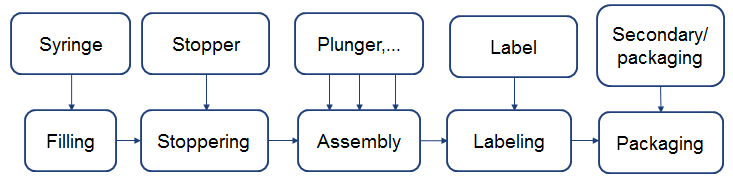
\includegraphics[height=4cm]{img/pfs_manu.PNG}
   \caption{Flowchart of the PFS manufacturing process.}
 \label{fgr:manu}
\end{figure}

\subparagraph{Syringe production}
It is necessary to coat the inner surfaces of the syringes with a layer of silicone. The silicone is either applied by spraying
silicone oil onto the glass or by coating the glass with a silicone emulsion that is baked onto the glass. A covalent atomic bond results in the barrel and the rest of the silicon oil is still freely movable thus less silicon oil is needed do reach a homogeneous distribution compared to spray siliconization[1]. Spray siliconization is applied with static nozzles and movable nozzles, which dive in the barrel providing a more homogeneous distribution. 
\subparagraph{Aseptic filling}
Pharmaceutical manufacturing companies that prefilled syringes may receive the syringes ready-to-use or as bulk syringes. Companies that choose to work with bulk syringes will clean, sterilize and apply silicone at their facilities. Ready-to use syringes are pre-cleaned, pre-sterilized and, if needed, siliconized.
The equipment can be paired with a variety of filling pumps. The types of filling pumps available include a diaphragm pump, rotary peristaltic pump, rotating piston pump and a time/pressure filler. All systems have their advantages and disadvantages.
\subparagraph{Stopper placement}
The goal is to place the stopper near the surface of the solution without touching the liquid. A gap of approximately 4$\pm$2mm is left between the solution and the surface of the plunger. Placement of the plunger closer to the solution risks the solution escaping around the edges of the plunger and leaving droplets of liquid between the ribs of the stopper, they are seated by one of two mechanisms. Vent-tube stoppering (see Figure \ref{fgr:stoppering} below) collects the plunger in stainless steel tubes that compress the plungers and a plunger insertion rod pushes the plunger into the syringe barrel. Compressing the plunger before placement allows air to escape around the plunger so that it will remain in place when it expands to fit into the barrel. 

\begin{figure}[h]	
	\centering
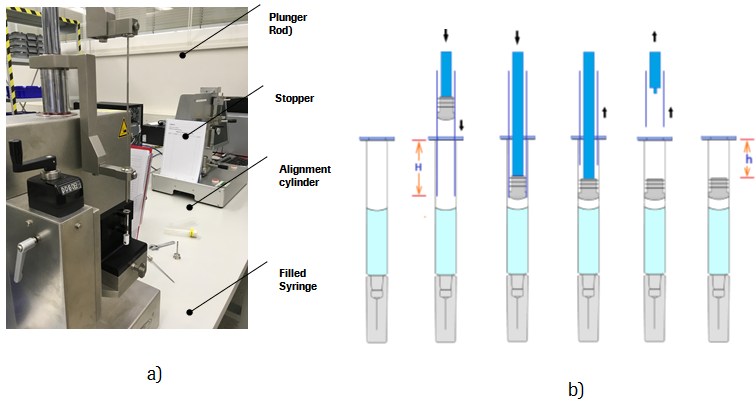
\includegraphics[height=6cm]{img/stoppering.PNG}
   \caption{a) Picture of the stoppering machine (B\&S) and b) scheme of the stoppering process.}
 \label{fgr:stoppering}
\end{figure}

%Vacuum stoppering operates with negative pressure to place the plungers. The stopper slides in the syringe barrel and stack up a silicon oil ring which has an influence to $d_{oil}$. Plungers are collected into a cylinder and the cylinder makes contact with the top of the syringe. A vacuum is pulled through the cylinder to remove air and the plunger is vacuumed out of the tube and into place in the barrel of the syringe. There are some syringes that are only compatible with vacuum plunger placement.

\subparagraph{Plunger assembly}
The plunger does not have to be connected with the stopper, as a matter of fact, designs exist without any plunger pin. However, disconnecting involves risking that the plunger might fall off if the PFS is turned upside down. Another common way of connecting the two is with a screw-in mechanics the assembly machine required thus torque and a mild downward movement.
The most common system is to place cameras. For assembly machine that check the distances, before and the insertion and if there are any gaps.
\begin{figure}[h]	
	\centering
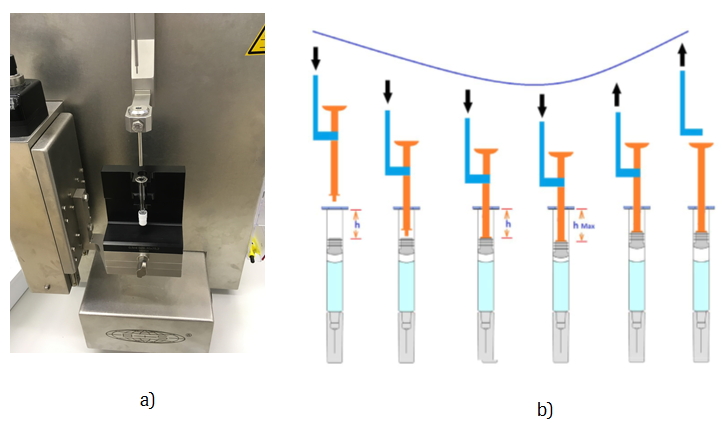
\includegraphics[height=7cm]{img/plungering.PNG}
   \caption{a) Picture of the stoppering machine (B\&S) and b) scheme of the plunger assembly process.}
 \label{fgr:PFS}
\end{figure}

\newpage
\subsection{Plunger assembly characterization}
The main measurement technique is with a tensile machine where the plunger is pushed by a stamp with is connect to a force sensor. Starting from the beginning: the plunger is lowered into the stopper until the plunger pin tip touches the inner walls of the stopper. The plunger starts the insertion by deforming the stopper walls pushing towards the exterior, thus increasing the contact area between the three components. This goes on until the pin is fully inserted into the stopper cavity, ending the first section of the force-displacement curve (see Figure \ref{fgr:force}). At this point the stopper and plunger have gained enough common surface area, allowing it to surmount the break loose force $F_{BL}$ necessary to overcome the static friction between barrel and stopper. This results in a sharp drop in force and a downwards displacement of the stopper. This movement causes the air bubble situated between the stopper and the medium to compress until the pressure is built up enough to compensate the static friction between the plunger and the stopper. This 2nd step is represented by curve in the force-displacement diagram and can also be derived theoretically with Boyle's law, as will be shown later. Once the air pressure is enough the insertion process continues, overcoming the maximum required force until the snap-in, which can be seen as a plateau and than a sharp drop. This gives a measurable parameter: the maximal force $F_{max}$.  Last but not least, if the compression continues the reaches a hard stop, given by the combination of the maximum compression of rubber, air, and liquid incompressibility.

The assembly can be divided in 4 stages as shown in the picture below:


\begin{figure}[h!]	
	\centering
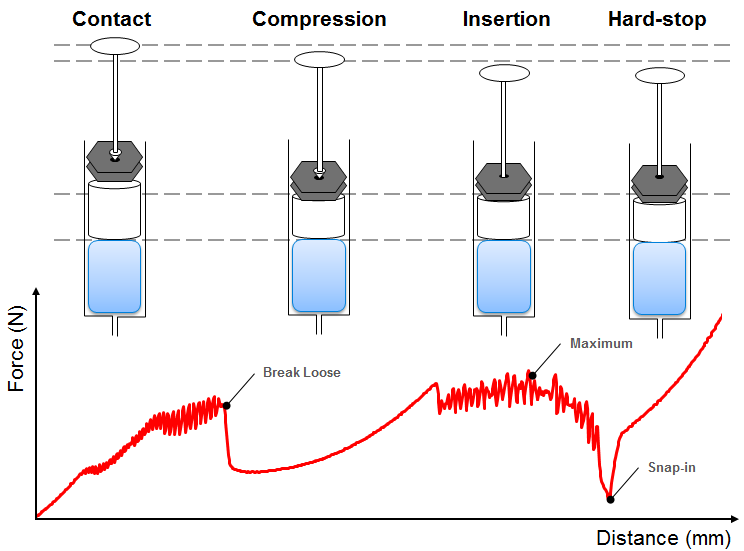
\includegraphics[height=9.5cm]{img/force.PNG}
   \caption{Plunger Assembly Step characterization}
 \label{fgr:force}
\end{figure}


\newpage
\subsection{Physical phenomena}
In order to fully comprehend the process it is necessary to study the single handedly. This next subsection I would like to give more detail on how these single phenomena affects the assembly.
Based on this analysis discuss what experiments are necessary to build the model. 
As seen above all steps have to some degree involved with material deformation, friction between the stopper-plunger and stopper-syringe with addition of air bubble compression in the second step.
The system is mainly friction dominated and thus this defines which component of the system is going to move: the plunger or the stopper.
In the following table the stages are shortly summarized and the involved phenomena.

\begin{table}[h]
\def\arraystretch{1.5}
\caption{Plunger assembly steps.}
	\begin{tabular}{l p{6cm}p{5cm}}
	Phase & Description & Acting Phenomena \\
    \hline
    1. Contact      & Plunger touches the stopper and compresses it & Hyperelastic deformation, Static Friction \\
    2. Compression  & Break loose: air bubble compression and stopper movement   & Dynamic friction, air pressure increase\\
    3. Insertion    & Given the air bubble pressure, the plunger is inserted until snap-in                         & Air pressure, Static friction\\
    4. Hard stop    & Further compression                           & Deformation, air pressure\\
    \hline
	\end{tabular}
\end{table}

\subsubsection{Deformation}
Rubber deformation, in contrast with other plastics and common polymers, is described by hyperelastic strain energy density laws. This is the case because rubber behaves similarly to elastic materials but is nonlinear. As such, there are a number of models which aim to describe the behavior for the different deformation modes of the material.
The stopper is going through different types of deformation during the assembly process. First, in the stoppering a concentric compression is applied in order to fit in the syringe cavity. Then, during the plunger insertion process, the walls are pushed to the side by the plunger pin which makes its way into the tube. Finally, at the snap-in the stopper reaches maximum strain.
\begin{figure}[h!]	
	\centering
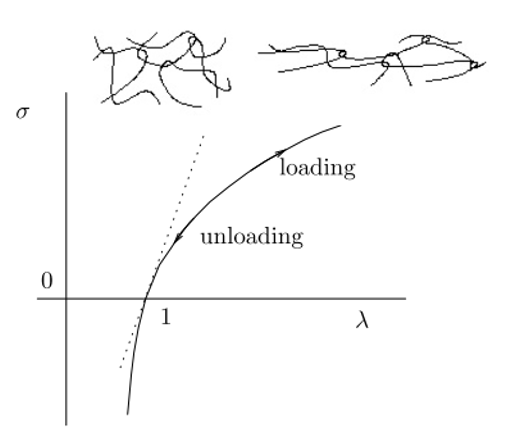
\includegraphics[height=3cm]{img/strainstress.PNG}
   \caption{PR Assembly Step Break-down}
 \label{fgr:PFS}
\end{figure}

\newpage
\subsubsection{Friction}
 There are many factor involved in this and they are represented below
As the picture below illustrates, the Ishikawa diagram
\begin{figure}[h!]	
	\centering
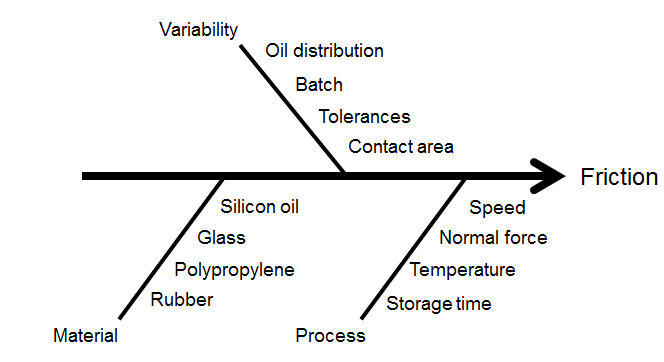
\includegraphics[height=7cm]{img/ishi.PNG}
   \caption{Strain stress curve and ishikawa for mat def}
 \label{fgr:PFS}
\end{figure}

\paragraph{Plastic - Rubber}
This interaction is defined by the materials which are Bromobutly rubber and polypropylene.
The surface is very rough leading to high friction coefficients
\paragraph{Rubber - Glass}
This is special because it is a wetted contact, namely by silicon oil. This is introduced to the system to allow the delivery and to lower the break loose force required. Thus, although relate to other factors such a speed and geometry break loose force is highly dependent on this silicon layer and has been thoroughly studied in the literature.
\begin{equation}
F_{friction}=\frac{\pi \cdot \mu \cdot l_{stopper} \cdot d_b}{d_oil}\cdot v
\end{equation}

\subparagraph*{Break-loose Force} 	The break-loose force is determined through the static friction between stopper and glass barrel respectively silicon oil layer. Is the maximum detected force to overcome the static friction between glass barrel and stopper. It is a special event in its movement  Once the BLF is overcome, the stopper begins to glide.
The break loose force ($F_{BL}$) is defined as the maximum force required to overcome the static friction between the stopper and the glass barrel.
\begin{equation}
F_{BL}=F_{friction}\frac{d_{b} \cdot l_b}{d_{b} \cdot l_{b}}
\end{equation}


\subsubsection{Air bubble compression}
The air bubble is in the system from the beginning and its volume and pressure is dependent on the stopper. 
The size of the bubble is defined by the space between the drug product and the stopper, this distance is called headspace.
This component is central to the plunger insertion as it provides the necessary reaction force to allow for it. However, this will only be the case if it is compressed enough. Unfortunately, the standard stopper placement technique is vent tubing, thus the bubble has air pressure of 1 atmosphere. Consequently, the stopper has to move in order for the bubble to build up enough pressure. The force applied by the air can be derived from Boyle's law. If we approximate the air column to a cylinder.
\begin{eqnarray}
p_1V_1=p_2V_2; p_2=p_1\frac{V_1}{V_2}\\
p_2=p_1\frac{h_1}{h_2}; V=\pi r^2 h\\
F=p_1\pi r^2 \frac{h_1}{h_2} with F=pA
\end{eqnarray}
$h$ is the headspace, p the pressure, V the volume, F the force, A the area, $r$ the radius of the syringe inner diameter. 
\begin{figure}[h!]	
	\centering
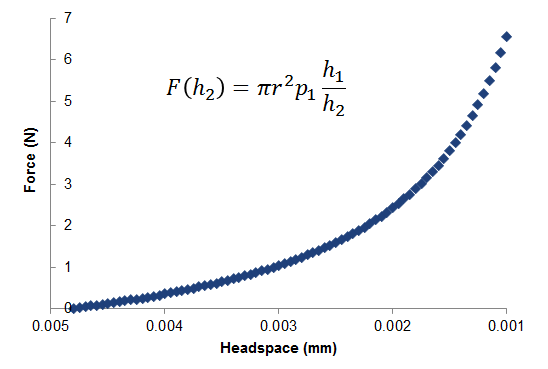
\includegraphics[height=7cm]{img/forceboyle.png}
   \caption{PR Assembly Step Break-down}
 \label{fgr:PFS}
\end{figure}

\newpage
\subsection{Parameter selection}

As described above the main phenomena are air bubble compression, rubber deformation and friction. Of the three aforementioned phenomena there are a number of factors that influence the plunger insertion and they are listed below. These can be studied with experiments and simulation.

\begin{figure}[h!]	
	\centering
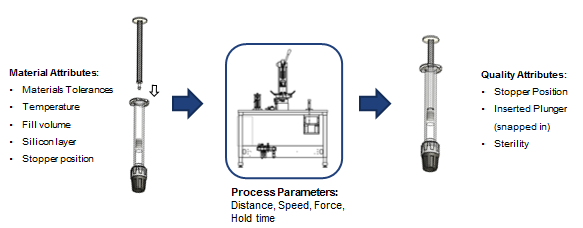
\includegraphics[height=5cm]{img/in_out.PNG}
   \caption{PR Assembly Step Break-down}
 \label{fgr:PFS}
\end{figure}
    
\subparagraph*{In-scope}
 
	Geometry is the most obvious category of parameters that potentially affect the the insertion force. The reason is contact area. Basically, the insertion is enabled by friction or rather a ratio between the plunger/stopper and stopper/glass barrel friction coefficients. Thus, any change in geometry that might increase of lower the contact area between the components I considered, of relevance are thus the plunger pin dimensions, like its length, diameter and cone angle and its negative fit geometry, the stopper inner tube length and diameter. Of importance are also the rip diameter of the stopper and	syringe diameter which determines the stopper compression. A bigger stopper has a bigger surface and the friction depends on the stopper size. Effect through $l_{stopper}$  ,$d_{barell}$
	 Plunger positions affect the variability of the measured syringes regarding to gliding forces[18].
	Environmental factors like temperature and humidity.
    Storage temperature and humidity affects the silicone oil viscosity and material aging. Therefore the material can be changed to slightly different characteristics and the silicon flows out faster. Effect to break loose force $\mu_{oil}$
    
    Friction can be studied as a results of actual forces and can be used as a bulk property in simulations. However, real experiments to determine the friction like roughness of materials or silicon oil inspection is considered out of scope. 
\subparagraph*{Out-of-scope}
Suppliers are NO and GB with different production sites.
Batch variability describes the fluctuations in different batches. 
	Different Materials like other silicone oil, different stoppers or different glasses affect the friction. 
	Vent-tube or vacuum stoppering are different stopper placement processes.  Vent-tube stoppering was applied for all investigated PFS. 
	Parameters of the silicon oil are out of scope thus, technique, oil distribution, its viscosity, interactions and amount
    

\begin{table}[h]
\def\arraystretch{1.5}
\caption{Potential process impact factors}
	\begin{tabular}{p{2 cm} p{2 cm} l l l}
	Category & Component & Factor (symbol) & Specification (unit)& Control  \\
    \hline
    Geometry& Barrel 	& Inner diameter $d_b$& 4.65 $\pm$ 0.1 mm& Caliber\\
    		& Stopper 	& Rib diameter	$d_r$& 5.00 $\pm$ 0.15 mm& CT-Scan\\
			& 			& Inner diameter$d_i$& 1.60 $\pm$ 0.25 mm& CT-Scan\\
            &			& Tube length	$d_l$& 3.20 $\pm$ 0.25 mm& CT-Scan\\
            &			& Position 		$x_s$& 4.87 $\pm$ 1.5 mm& Scale\\
			& Plunger	& Pin diameter	$d_p$& 2.00 $\pm$ 0.07 mm& Scale\\
            &			& Pin length	$x_l$& 5.10 $\pm$ 0.2 mm& Scale\\
    Friction& Silicon oil (stopper, barrel)& Friction coefficient $f_l$&				&	\\
            & (plunger, stopper)& Friction coefficient $f_l$ &				&	\\
  Assembly Parameters&Assembly machine	& Displacement	$x_i$& 6 $\pm$ 4 mm& Computer\\
   					&					&Insertion Speed	$v_i$		& 750 $\pm$ 745 mm/min& Computer\\
                    &					& Hold time	$t_h$	& 2.5 $\pm$ 2.5 s	& Computer\\
  Environment& Ambient Air		& Temperature $T$& 20 $\pm$ 3 $^{\circ}$C & Thermometer\\
   					&					&Humidity	$p$		& 1 $\pm$ 745 atm& hygrometer 
    \end{tabular}
\end{table}

\begin{figure}[h!]	
	\centering
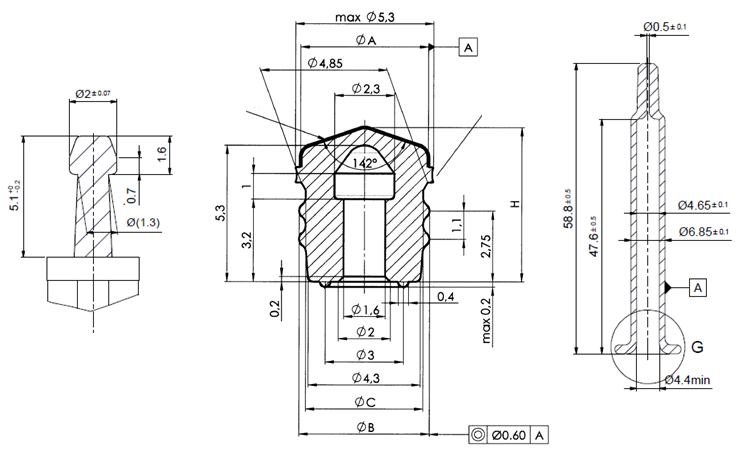
\includegraphics[height=7cm]{img/blueprint.PNG}
   \caption{Blueprints of syringe, stopper and plunger with evidenced components that affect the process}
 \label{fgr:PFS}
\end{figure}

\newpage
\subsection{Testing strategy}
Based on the previous considerations here is a list of experiments where factors have to be discerned and data necessary to be generated.

\begin{figure}[h!]	
	\centering
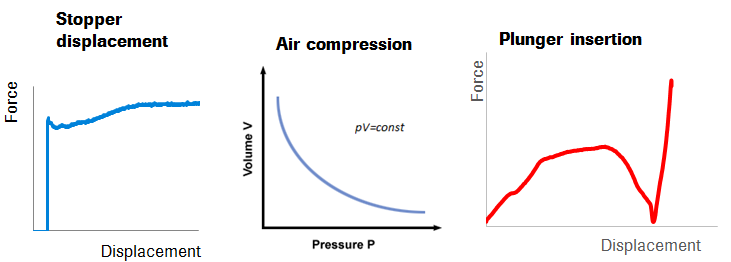
\includegraphics[height=5cm]{img/tests.PNG}
   \caption{Testing strategy}
 \label{fgr:PFS}
\end{figure}

Assume the following are constant: air bubble pressure, water viscosity, silicon oil properties (layer) assembly machine parameters (?), a storage temperature of 25 deg of 3 months